\chapter{Set Up and Method}
\label{ch:5}

\section{Technical Environment}

The experiments carried out in this thesis were executed in Google Colaboratory (Colab) which is a Google-hosted implementation of Jupyter Notebook\cite{72-GoogleColaboratory,73-ProjectJupyter}. 
The base components of a Notebook are cells that can be grouped thematically. 
The cells can contain code or markdown, smoothing out the transition between coding and writing which is conducive to a smooth workflow.
Another key advantage of this setup is the ability to work from anywhere. This is possible as the notebook is being executed by Google's cloud servers; there were no specific hardware dependencies for the computations. 

Given the choice to work in the Jupyter environment, Python becomes the natural choice of programming language\cite{74-WelcomePython}. 
This choice is further substantiated by the prevalence of existing modules made for data analysis.
There are significant computational gains from using an extension of Python called Cython\cite{75-CythonBest}. 

We used the module \mintinline{Python}{trajectory_distance}\cite{43-TrajectoryDistance} to compute almost all the distance functions. 
There were no implementations of Euclidean Distance and Move-Split-Merge, so we coded our own. 
The former was trivial to implement.
As for the latter, the creators of MSM had published a JAVA implementation of their algorithm. 
Using that code as a guide we created a “Pure-Python”-Cython cell in the Jupyter Notebook which was used for its similarity distance computation.  
Due to the differences in implementation, we cannot evaluate the algorithms’ time complexity fairly.


\clearpage
\section{Data Set}
In this thesis, the aim is to gain information about various similarity measures and consequently, the setup should be as data set agnostic as possible.
With this in mind, we first generated synthetic data for initial test runs and then modified real trajectory data which we could use for more extensive tests.

% This is in part because there could be some underlying similarities that are. It is hard to with synthetic data, and the advantage of using real data is that we may gain insight from it.  As far as deciding on which data set we will use, the decision has not been made yet. Currently there are two data sets that seem interesting enough to examine more closely.  




\subsection{Synthetic Trajectory Generation}

% The motivation behind using a synthetic data set first is so that it is possible to have control over the input data while getting started. Primarily we wish to ensure that the size of the data set is not too large as both clustering and the similarly measures could take a lot of computing time. Ideally we would have just a handful of trajectories for the first clustering jobs, as well as limiting the length of the initial trajectories. Real data sets could have many hundreds of trajectories and/or hundreds of values per trajectory and are therefore not well suited for early testing.


The generation of synthetic data was the first step of this experiment. 
The aim of doing this  was so that we could determine the architecture of the experiment validate that the distance functions were producing reasonable results.  
% When generating the trajectories, the data format was intentionally identical to that of the real data set. 
The generated data set can be seen in \Cref{fig:synthetic-data}. 
It quickly became evident that the data was too random to serve as a basis for the similarity algorithms.
Rather than using more advanced methods for creating synthetic data such that it could potentially accurately represent a complex system, we chose to examine trajectory real data.
 


\begin{figure}
\centering
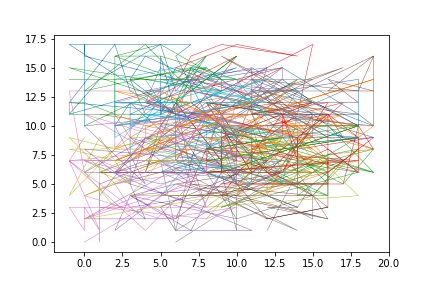
\includegraphics[width=.7\textwidth]{figs/traj/SYNTHETIC.png}
\caption{Synthetic data set of randomly generated trajectories.}
\label{fig:synthetic-data}
\end{figure}



\subsection{Real Trajectory Preprocessing}

The data set that was selected for this thesis is a taxi trajectory data set with  over 1.7 million rows\cite{3-TaxiTrajectory}. 
In addition to a large number of rows, there were superfluous columns such as what type of taxi ride it was and whether or not the trip was on a weekend. 
The first step of the data preprocessing was to remove these attributes from the rows.  
Next, a random subset consisting of just over 500 trajectories was selected. 
They were given unique IDs their routes can be seen in \Cref{sfig:real-med}. 


\clearpage
As mentioned in the \Cref{ch:3}, the Euclidean distance may only evaluate trajectories of the same length. 
Rather than interpolate to add data points– or compute the information gain of the trajectory elements and then get rid of the least informative ones, we truncated all trajectories to the same length. 
Moreover, initial tests indicated that a set of 500 trajectories was still too voluminous and time consuming to analyze. '
As a result, we created two subsets of those 500 raw trajectories, one significantly smaller than the other so that tests could be run quickly. The truncated trajectory sets are depicted in \Cref{sfig:real-trunc,sfig:real-trunc-mini}


% em dash  –

As seen in \Cref{fig:real-datasets} the trajectories are fairly spread out, and so we normalized the range of the coordinates of the data set.
We scaled the data so that they would be in the same value range and we could examine similarity on a seemly arbitrary set of lines. '
Without this step, trajectories spanning a small identical geographical area would artificially receive a higher similarity score by being near each other, regardless of shape similarity.
This is the re-scaling disconnected data from their real world source while maintaining a general similarity shape from trajectories that followed the same roads. 
Finally, we remark that the re-scaling was done with simplification of independently scaling the latitudinal and longitudinal dimensions, further distorting their relation to the underlying road network. 
The final scaled data set is graphed in \Cref{fig:scl-datasets}.


\begin{figure}[h!]
\centering
\begin{subfigure}{.451\textwidth}
    \centering
    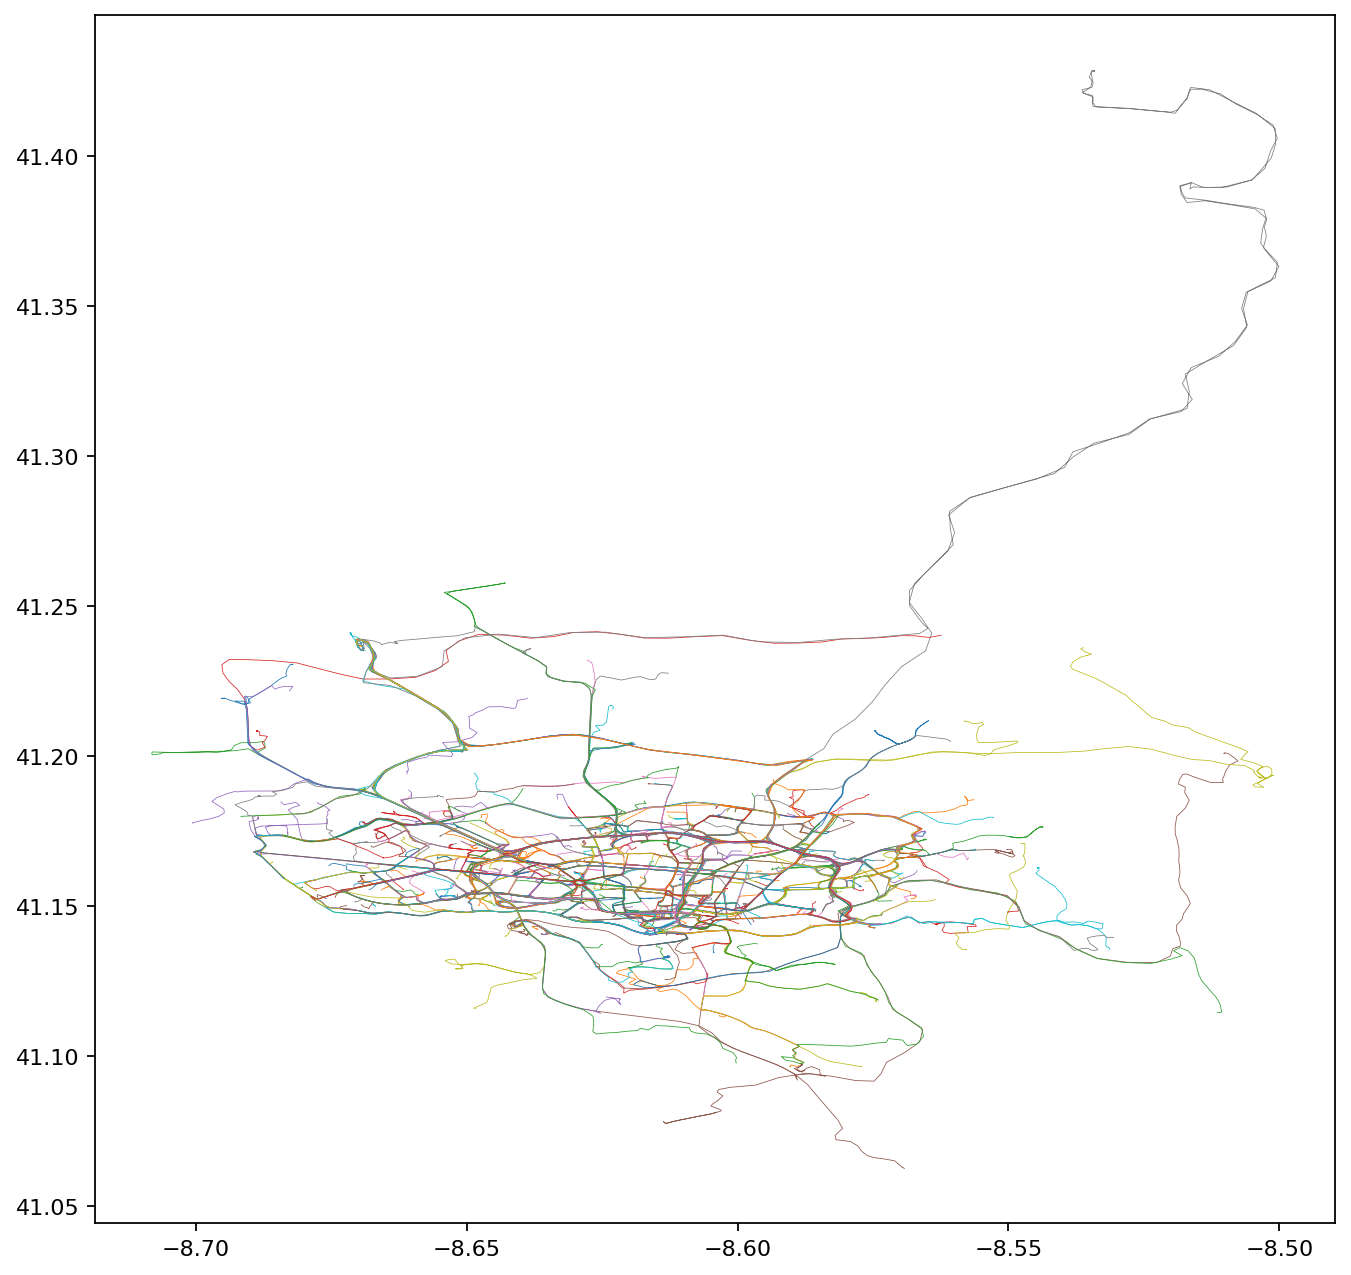
\includegraphics[width=\textwidth]{figs/traj/REAL_MED.png}
    \caption{Subset with 551 entries}
    \label{sfig:real-med}
\end{subfigure}
\hfill
\begin{subfigure}{.451\textwidth}
    \centering
    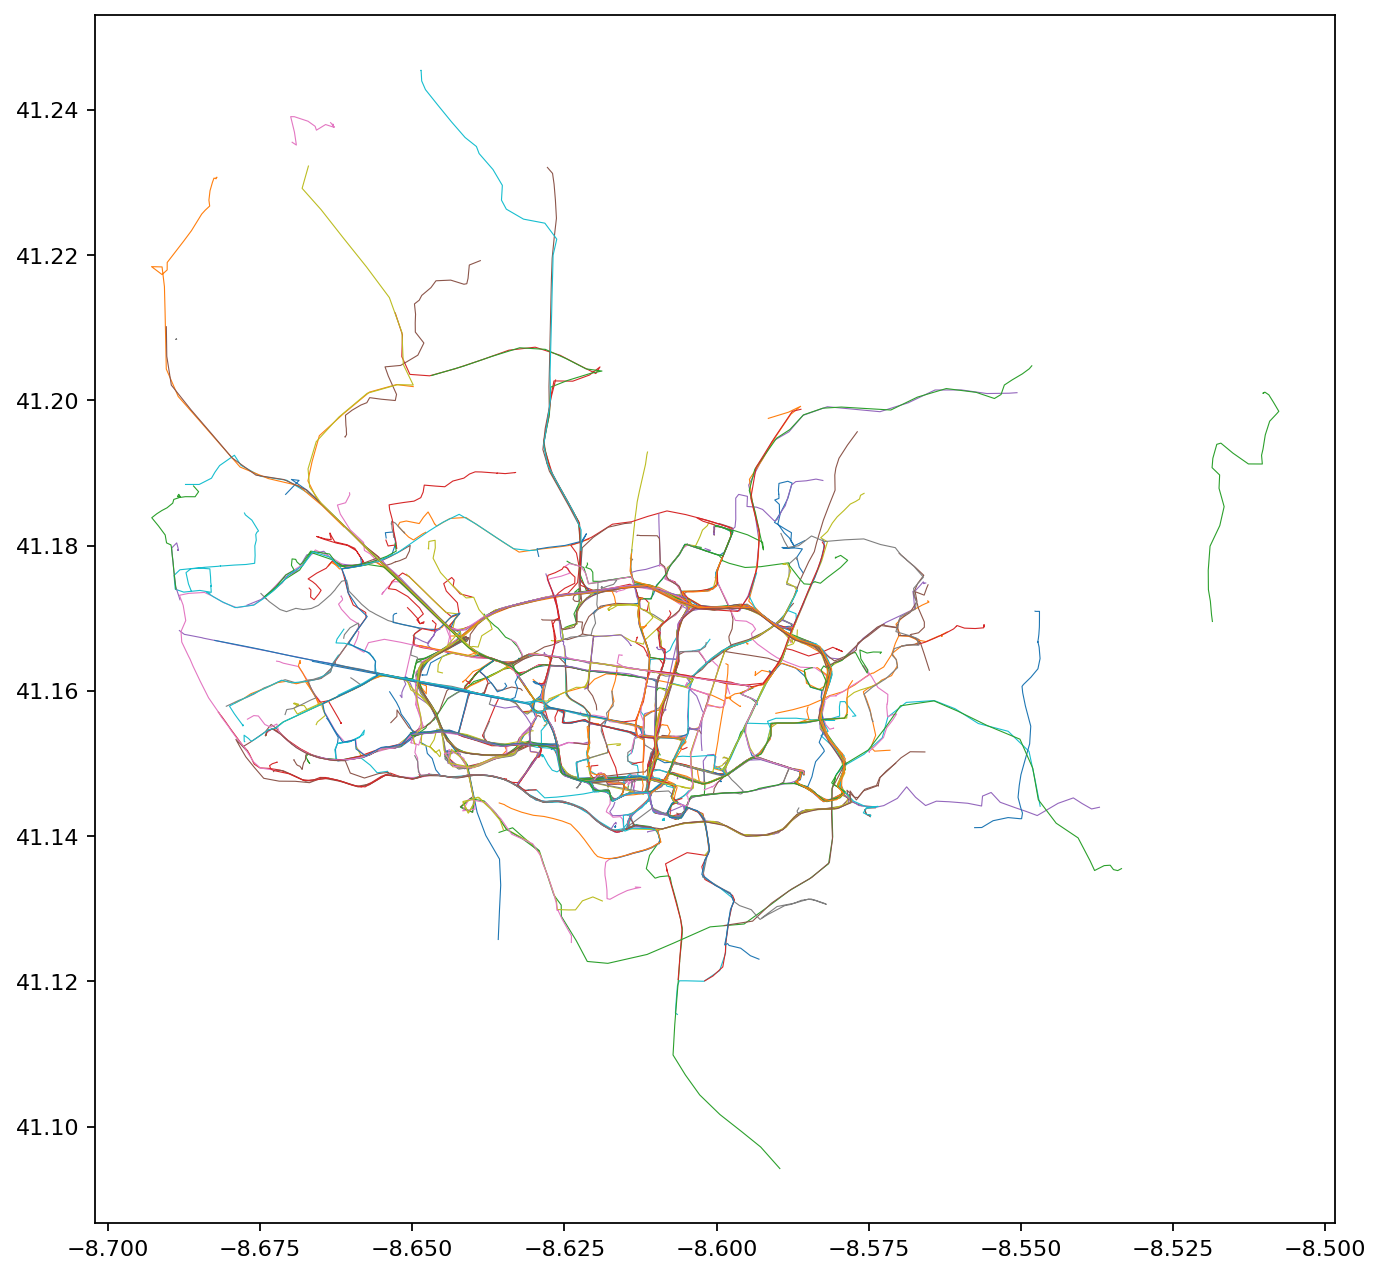
\includegraphics[width=\textwidth]{figs/traj/REAL_TRUNC.png}
    \caption{Truncated subset, 353 entries}
    \label{sfig:real-trunc}
\end{subfigure}
\begin{subfigure}{.451\textwidth}
    \centering
    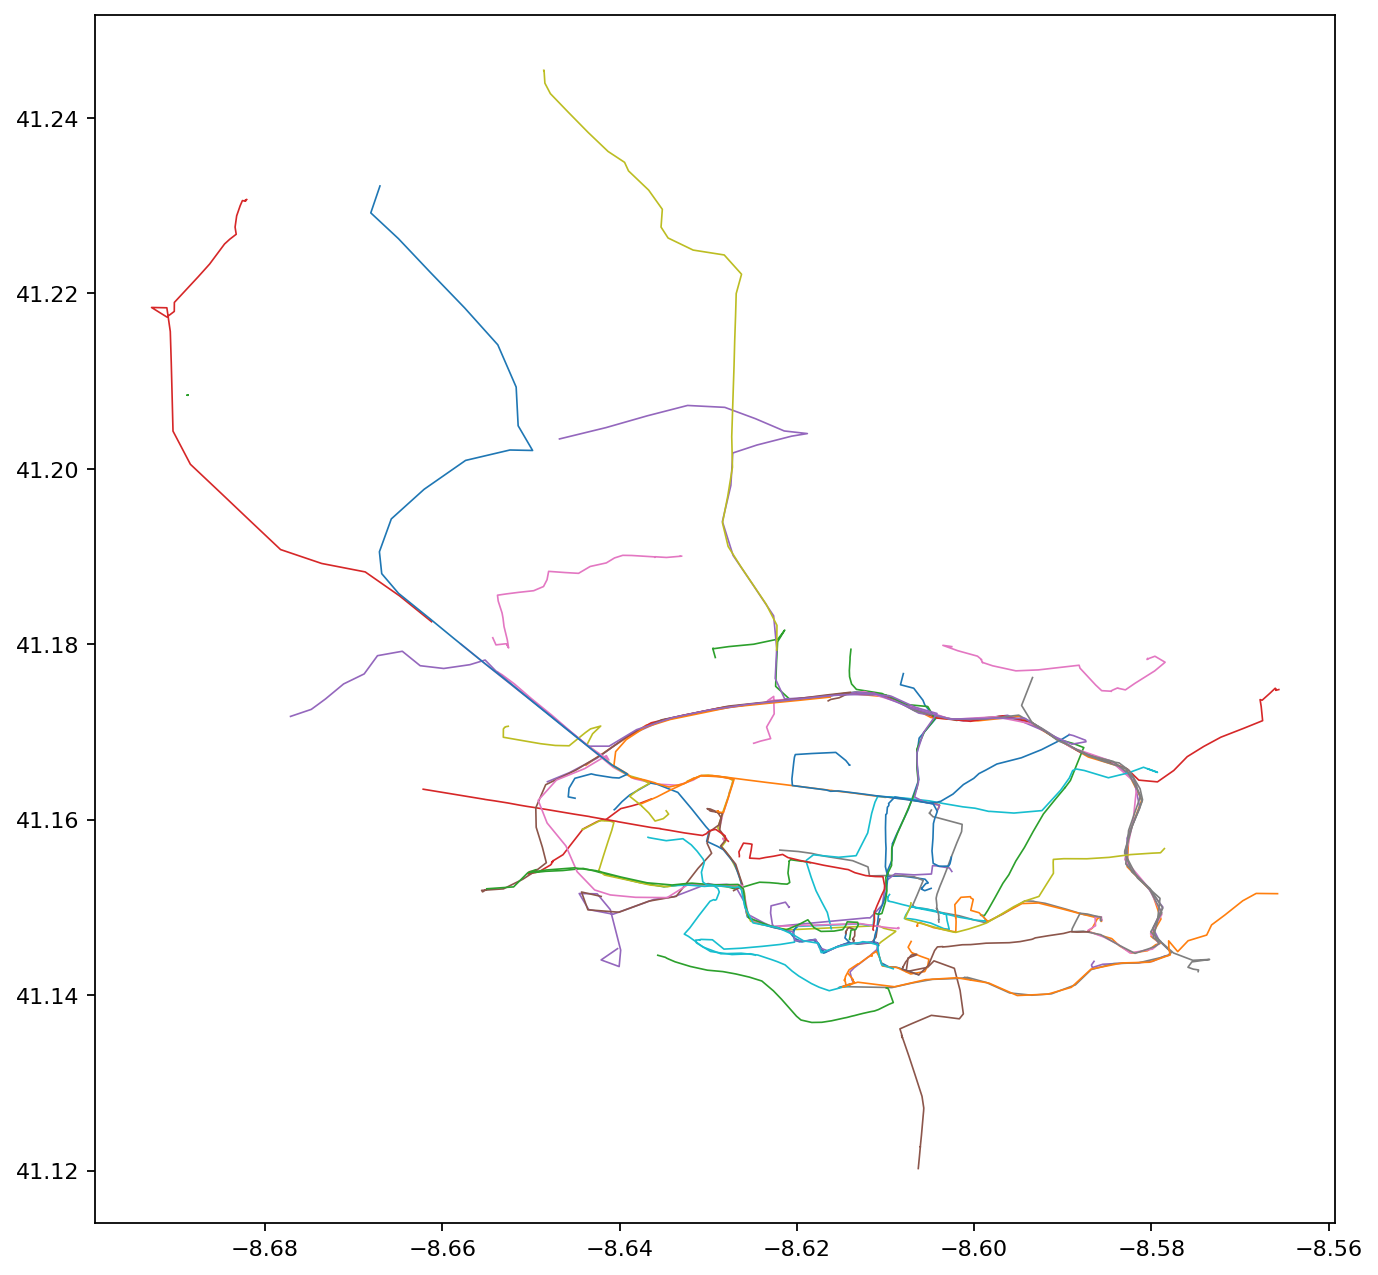
\includegraphics[width=\textwidth]{figs/traj/REAL_TRUNC_MINI.png}
    \caption{Subset of the truncated data with 53 entries}
    \label{sfig:real-trunc-mini}
\end{subfigure}
\caption{Real data set with trajectories collected from taxis}
\label{fig:real-datasets}
\end{figure}


\begin{figure}[h!]
\centering
\begin{subfigure}{.45\textwidth}
    \centering
    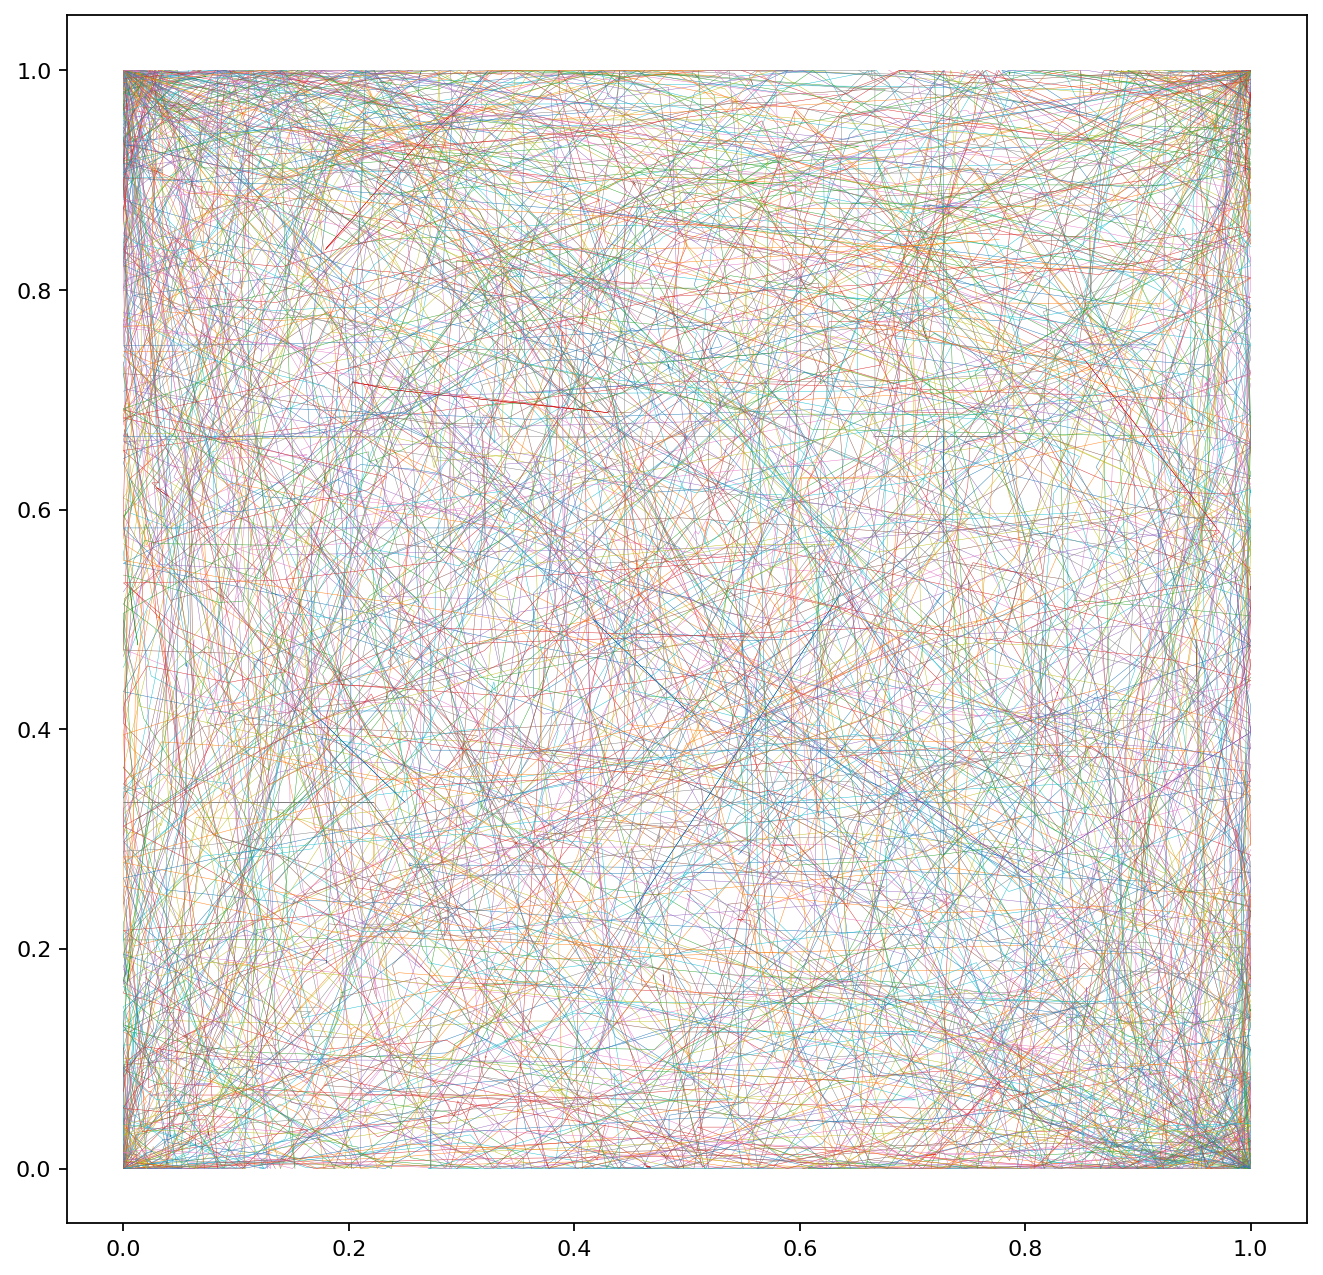
\includegraphics[width=\textwidth]{figs/traj/REAL_TRUNC_SCL.png}
    \caption{Scaled version of the data set in \newline\Cref{sfig:real-trunc}}
\end{subfigure}
\hfill
\begin{subfigure}{.45\textwidth}
    \centering
    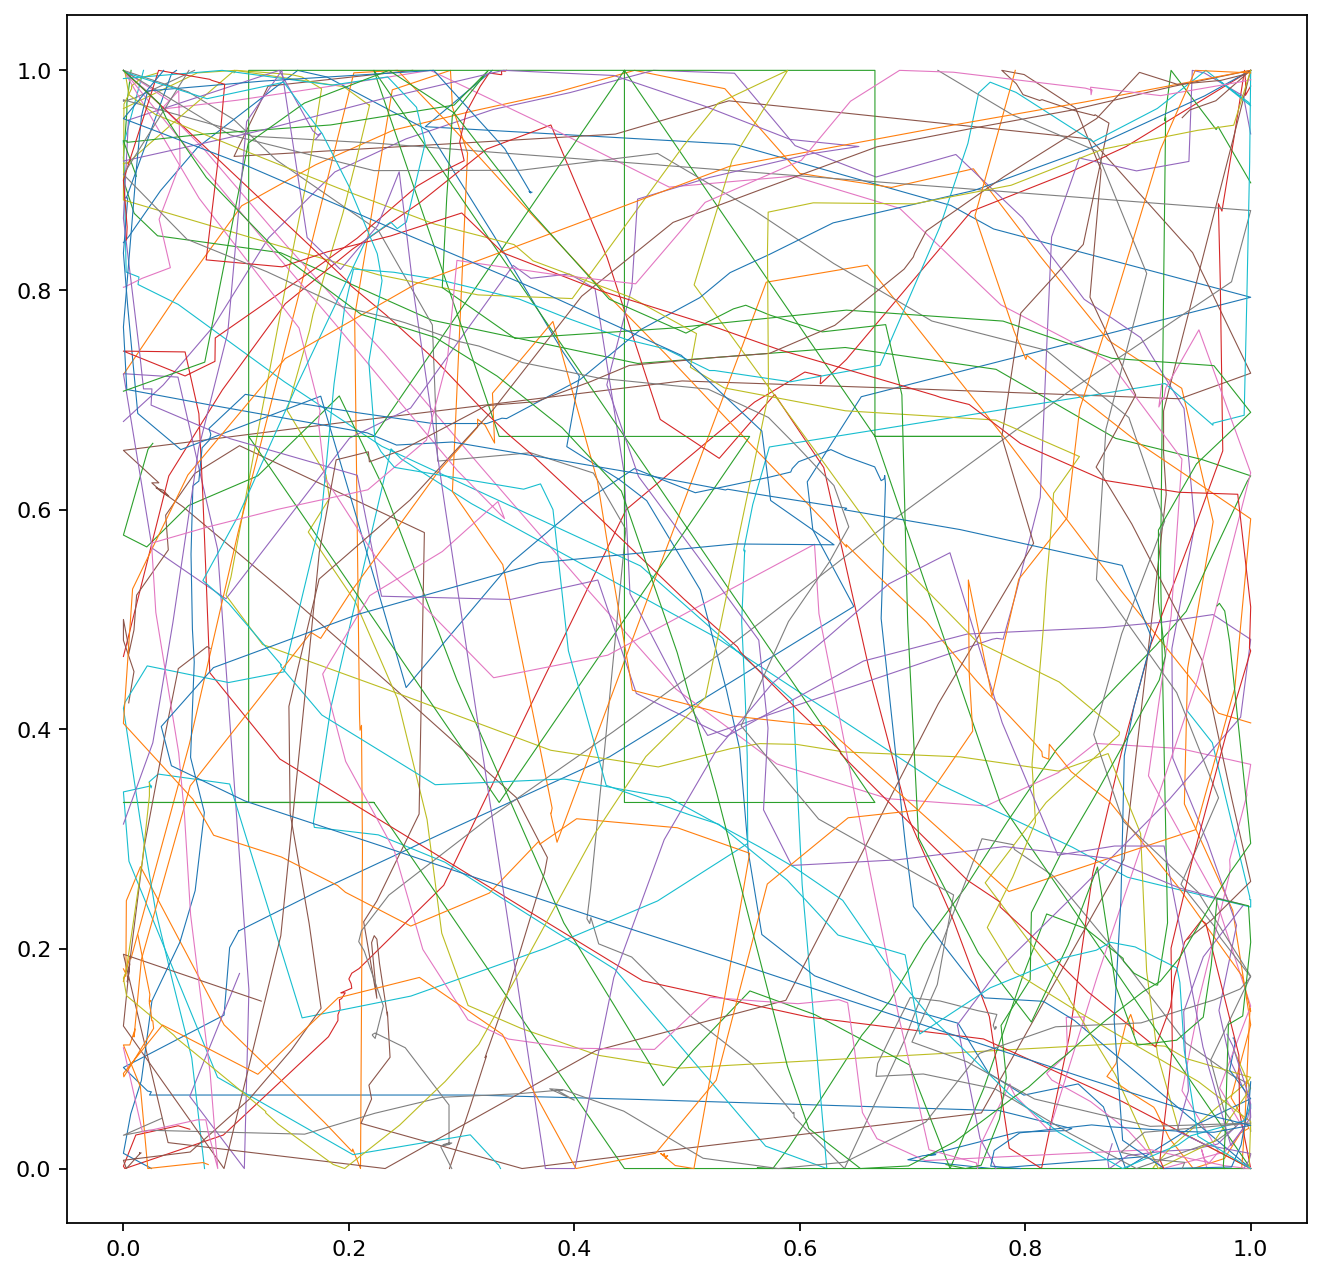
\includegraphics[width=\textwidth]{figs/traj/REAL_TRUNC_SCL_MINI.png}
    \caption{Scaled version of the data set in\newline \Cref{sfig:real-trunc-mini}}
\end{subfigure}
\caption{The trajectories in the data set after re-scaling}
\label{fig:scl-datasets}
\end{figure}



\section{Setting Parameter Values}

Three of the measures required a parameter value. 
For each of the measures, we followed the guidelines that the original creators set for determining a fitting value.
While the value may have been usable for our tests, we did not fully optimize any of the parameters for this specific data set. 
This may have negatively impacted their performance, and as a counter, we would test more than one value where we could reasonably determine another value. 
For details regarding parameters themselves, refer to \Cref{ch:2}. 


\subsection{EDR}

The creators of this method explicitly stated that they achieved the best clustering results when the matching threshold $\epsilon$ was set to a quarter of the maximum standard deviation\cite{12-RobustFast}. 
The time-series data that were used in their research were one-dimensional, thus finding the standard deviations of each series was a straightforward task.
Akin to how to how the re-scaling was done, a naive process that isolated the two dimensions was used to estimate a sensible value for $\epsilon$. 
For each trajectory, the standard deviation of each dimension was calculated.
Then the mean of the largest standard deviations from the data set was computed.
A quarter of that value was used as the first value of $\epsilon$, while the second value was half; the two values we used for EDR were $\{0.101, 0.203\}$

\clearpage
\subsection{ERP}
The researchers that developed ERP stated that the algorithm would be a metric as long as the reference value, $g$, was fixed\cite{13-MarriageLpnorms}.

In their paper, they asserted that fixing $g$ at the origin was a natural choice. 
Consequently, we set $g = (0, 0) $ for the tests in this set up. 
We did not try another value for $g$ due to there being a lack on information of how approximate another suitable value.

% em dash  –

\subsection{MSM}
Much like the creators of the algorithm– and subsequent experiments of MSM \cite{40-MoveSplitMergeMetric, 42-GreatTime, 52-OnlineEfficient}, we let the cost, $c$, vary over different orders of magnitude. 
Concretely $c$ took the values  $\{1, 0.1, 0.01\}$.
These orders of magnitude were chosen based on the results from initial tests executed on the subset of truncated trajectories.  

% \section{Condensed Similarity Matrices}
% Most of these methods were readily implemented in an existing python module \cite{43}. More about implementation in \Cref{ch:5}.


\section{Clustering Analysis}
\label{sec:5-clustering}

% All similarity distances but MSM were computed using an existing python library\cite{43-TrajectoryDistance} for trajectory similarity. In order to compute the MSM similarity distance we adapted the JAVA implementation for $1-$dimensional time-series data that its creators had published. 
The first step was to compute all pairwise trajectory similarity scores using each of the similarity distance functions. 
The next step was to create the clusters and as specified in \Cref{ch:2}  two different models were used for this. Details on the clustering models were given in that chapter as well. 

The Python's module \mintinline{Python}{sklearn} contains functionality for creating for both types of clustering, as well as models for even more options.  
The module can take parameters which affect how the model creates the clusters. An example would be setting an iteration limit for affinity propagation. 
However,  in keeping this stage of the experiment as simple as possible, all but one parameter value were kept their defaults.


The value we specified was the number of clusters that the hierarchical model should create.
This was necessary as the stopping criterion for agglomerative clustering is to have one cluster that contains all elements.
The number chosen was for all intents and purposes arbitrary, but we set it to be the least number of clusters found by affinity propagation. 
Our motivation for picking this number, and keeping it equal for all measures, was that we wanted to have clusters of meaningful sizes while still being able to spot the variances from a given measure. 

Finally, we implemented a version of the Davies-Bouldin Index. 
Again, the underlying theory is elaborated upon on \Cref{ch:2}. 
The DB-index depends on having a representative observation of each cluster. 
Commonly this is either the center of a cluster or an exemplar observation that is the one nearest to other ones. 
Unfortunately, the center of a cluster of series data does not let itself be computed easily– especially in the cases where the trajectories are of unequal length. Furthermore, determining the exemplar observation would require us to pick a similarity to be the proper one.   

Yet again simplifications were made, and the center trajectory of a cluster was set to be the series of mean positions of all trajectories in that cluster.
The mean was computed in a lock-step manner using the $L_2$-norm. 
For the similarity distance computations necessary for the DB-index calculation, the Euclidean distance was used because of if the simplest one. 




% Once the parameters had been set and the data pre-processed the condensed similarity matrices were computed. With the pairwise distance between all trajectories computed we looked into the performance of each measure by applying two different clustering tasks: affinity propagation and hierarchical agglomerative clustering. The theory of the two clustering techniques are elaborated upon in [ref CHAPTER]. Scikit and sklearn models for clustering [CITE] were used for the generation of clusters.  

												

% For the hierarchical clustering, we used sklearn [CITE]’s Agglomerative Clustering model to compute the clusters and SCIPY’s cluster hierarchy methods display them. Complete linking – using a set number of clusters. An arbitrary number of final clusters were chosen, and in this case, that number was the smallest number of clusters that were found in the affinity propagation method. 

% The number of clusters should be large enough to capture the variance of possible final clusters, yet not so large that it would hinder meaningful groupings. 



% The Davies–Bouldin index was calculated by defining “separation of clusters” and “tightness within clusters” much like the authors of\cite{50-ReviewPerspective}. See CHAPTER for more details on the index and EQ for implementation specification. 
 




\section{Simplifications}

As stated at various points throughout the chapter, we made simplifications while setting up our experiment. 
The simplifications were made in order to limit the scope, and in some cases due to the time constraints surrounding the thesis. 
We close the chapter by summarizing them below. 


\begin{itemize}

\item The trajectories were truncated to equal length and then re-scaled so that they did not remain true to their original relative location. 

\medskip
\item At several points, longitude and latitude were treated as if they were independent series. 
This becomes particularly important with respect to re-scaling and cluster evaluation.

\medskip
\item At the evaluation stage, point-point distances, and trajectory-trajectory were calculated using the Euclidean distance. 
This further exaggerated the biases of the DB-index. 

\medskip
\item Clustering itself lacks a well-defined standard, meaning it is not necessarily the most appropriate application comparison.
\medskip

% the decisions to approximate the conversion 

\end{itemize}

The effect of simplification and the importance of the cluster evaluation is further elaborated upon in \Cref{ch:7}.





